%
%===============>>  ГРУППА 10-1 МОДУЛЬ 5  <<=============
%
\setmodule{5}

%BEGIN_FOLD % ====>>_____ Занятие 1 _____<<====
\begin{class}[number=1]
	\begin{listofex}
		\item
		\begin{minipage}[t]{\bodywidth}
			На рисунке изображён график функции вида \[ f(x)=ax+|bx+c|+d, \] где \(a, b, c, d\) --- целые числа. Найдите корень уравнения \(bx+c=0\).
		\end{minipage}
		\hspace{0.02\linewidth}
		\begin{minipage}[t]{\picwidth}
			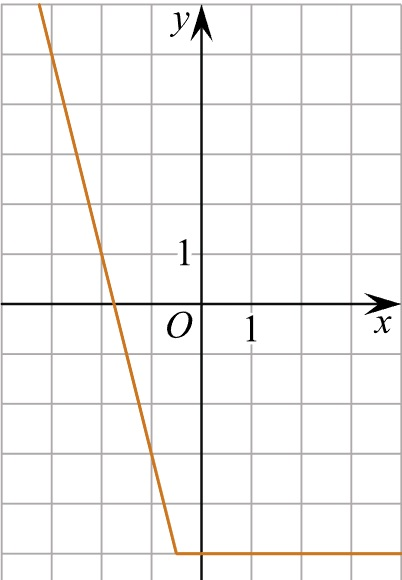
\includegraphics[align=t, width=\linewidth]{\picpath/G101M4H2-6}
		\end{minipage}
		\item
		\begin{minipage}[t]{\bodywidth}
			На рисунке изображён график функции вида \[ f(x)=ax-|bx+c|+d, \] где \(a, b, c, d\) --- целые числа. Найдите корень уравнения \(ax=d\).
		\end{minipage}
		\hspace{0.02\linewidth}
		\begin{minipage}[t]{\picwidth}
			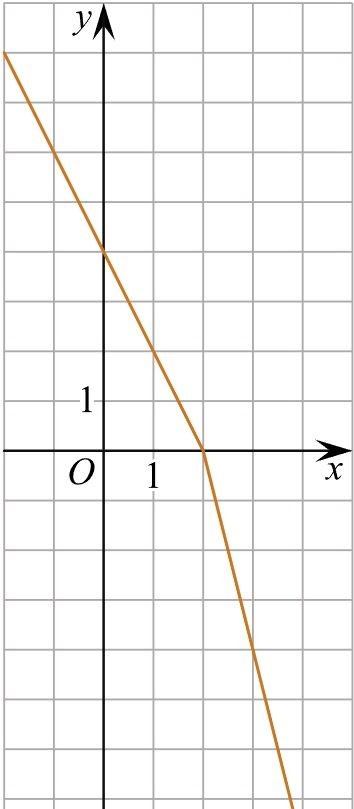
\includegraphics[align=t, width=\linewidth]{\picpath/G101M4H2-7}
		\end{minipage}
		\item
		\begin{minipage}[t]{\bodywidth}
			На рисунке изображён график функции вида \[ f(x)=ax+|bx+c|+d, \] где числа \(a, b, c, d\) --- целые. Найдите корень уравнения \(-ax-3d=10\).
		\end{minipage}
		\hspace{0.02\linewidth}
		\begin{minipage}[t]{\picwidth}
			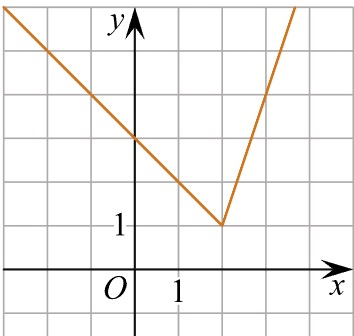
\includegraphics[align=t, width=\linewidth]{\picpath/G101M4C5-7}
		\end{minipage}
%				\item
%		\begin{minipage}[t]{\bodywidth}
%			На рисунке изображён график функции вида \[ f(x)=ax+|bx+c|+d, \] где числа \(a, b, c, d\) --- целые. Найдите корень уравнения \(bx+2c=1\).
%		\end{minipage}
%		\hspace{0.02\linewidth}
%		\begin{minipage}[t]{\picwidth}
%			\includegraphics[align=t, width=\linewidth]{\picpath/G101M4L7-6}
%		\end{minipage}
		\item Два велосипедиста одновременно отправляются в \( 60 \)-километровый пробег. Первый едет со скоростью на \( 10 \) км/ч большей, чем второй, и прибывает к финишу на \( 3 \) часа раньше второго. Найдите скорость велосипедиста, пришедшего к финишу вторым.
	\end{listofex}
\end{class}
%END_FOLD

%BEGIN_FOLD % ====>>_____ Занятие 2 _____<<====
\begin{class}[number=2]
	\begin{listofex}
		%1
		\item
		\begin{minipage}[t]{\bodywidth}
			На рисунке изображён график функции вида \[ f(x)=ax-|bx+c|+d, \] где числа \(a, b, c, d\) --- целые.\\ Найдите корень уравнения \(ax+d=19\).
		\end{minipage}
		\hspace{0.02\linewidth}
		\begin{minipage}[t]{\picwidth}
			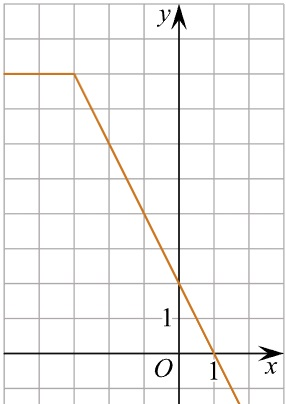
\includegraphics[align=t, width=\linewidth]{\picpath/K-L8}
		\end{minipage}
		%2
		\item
		\begin{minipage}[t]{\bodywidth}
			На рисунке изображён график функции вида \[ f(x)=ax+|bx+c|+d, \] где числа \(a, b, c, d\) --- целые.\\ Найдите корень уравнения \(bx+c=0\).
		\end{minipage}
		\hspace{0.02\linewidth}
		\begin{minipage}[t]{\picwidth}
			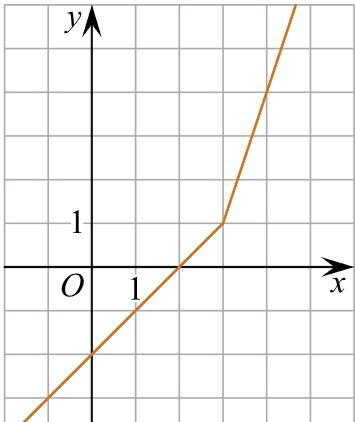
\includegraphics[align=t, width=\linewidth]{\picpath/K-L2}
		\end{minipage}
		%3
		\item
		\begin{minipage}[t]{\bodywidth}
			На рисунке изображён график функции вида \[ f(x)=ax+|bx+c|+d, \] где числа \(a, b, c, d\) --- целые.\\ Найдите корень уравнения \(ax+d=19\).
		\end{minipage}
		\hspace{0.02\linewidth}
		\begin{minipage}[t]{\picwidth}
			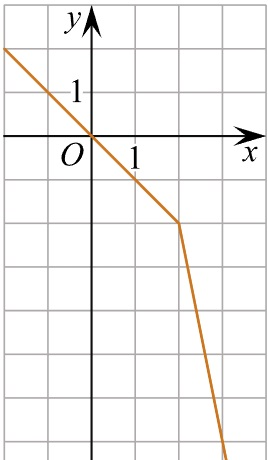
\includegraphics[align=t, width=\linewidth]{\picpath/K-L7}
		\end{minipage}
		%4
		\item
		\begin{minipage}[t]{\bodywidth}
			На рисунке изображён график функции вида \[ f(x)=ax-|bx+c|+d, \] где числа \(a, b, c, d\) --- целые.\\ Найдите корень уравнения \(ax=d\).
		\end{minipage}
		\hspace{0.02\linewidth}
		\begin{minipage}[t]{\picwidth}
			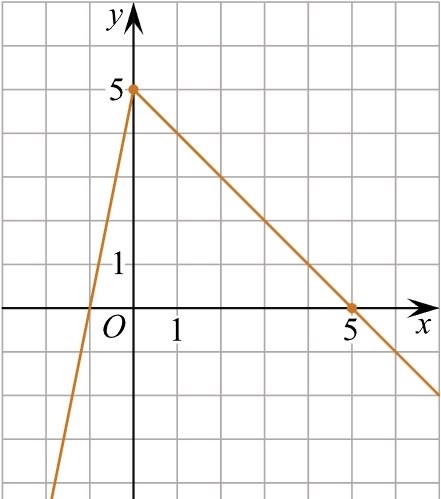
\includegraphics[align=t, width=\linewidth]{\picpath/K-L10}
		\end{minipage}
	\end{listofex}
\end{class}
%END_FOLD

%BEGIN_FOLD % ====>>_____ Занятие 3 _____<<====
\begin{class}[number=3]
	\begin{listofex}
		\item Занятие 3
	\end{listofex}
\end{class}
%END_FOLD

%BEGIN_FOLD % ====>>_____ Занятие 4 _____<<====
\begin{class}[number=4]
	\begin{listofex}
		\item Занятие 4
	\end{listofex}
\end{class}
%END_FOLD

%BEGIN_FOLD % ====>>_____ Занятие 5 _____<<====
\begin{class}[number=5]
	\begin{listofex}
		\item Занятие 5
	\end{listofex}
\end{class}
%END_FOLD

%BEGIN_FOLD % ====>>_____ Занятие 6 _____<<====
\begin{class}[number=6]
	\begin{listofex}
		\item Занятие 6
	\end{listofex}
\end{class}
%END_FOLD

%BEGIN_FOLD % ====>>_____ Занятие 7 _____<<====
\begin{class}[number=7]
	\begin{listofex}
		\item Занятие 7
	\end{listofex}
\end{class}
%END_FOLD

%BEGIN_FOLD % ====>>_ Домашняя работа 1 _<<====
\begin{homework}[number=1]
	\begin{listofex}
		%1
		\item Из одной точки круговой трассы, длина которой равна \(14\) км, одновременно в одном направлении стартовали два автомобиля. Скорость первого автомобиля равна \(80\) км/ч, и через \(40\) минут после старта он опережал второй автомобиль на один круг. Найдите скорость второго автомобиля. Ответ дайте в км/ч.
		%2
		\item На изготовление \(475\) деталей первый рабочий тратит на \(6\) часов меньше, чем второй рабочий на изготовление \(550\) таких же деталей. Известно, что первый рабочий за час делает на \(3\) детали больше, чем второй. Сколько деталей в час делает первый рабочий?
		%3
		\item
		\begin{minipage}[t]{\bodywidth}
			На рисунке изображён график функции вида \[ f(x)=ax-|bx+c|+d, \] где числа \(a, b, c, d\) --- целые.\\ Найдите корень уравнения \(ax=d\).
		\end{minipage}
		\hspace{0.02\linewidth}
		\begin{minipage}[t]{\picwidth}
			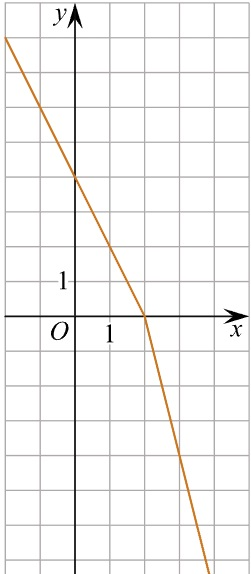
\includegraphics[align=t, width=\linewidth]{\picpath/K-L9}
		\end{minipage}
		%4
		\item
		\begin{minipage}[t]{\bodywidth}
			На рисунке изображён график функции вида \[ f(x)=ax+|bx+c|+d, \] где числа \(a, b, c, d\) --- целые. Найдите корень уравнения \(ax+2d=12\).
		\end{minipage}
		\hspace{0.02\linewidth}
		\begin{minipage}[t]{\picwidth}
			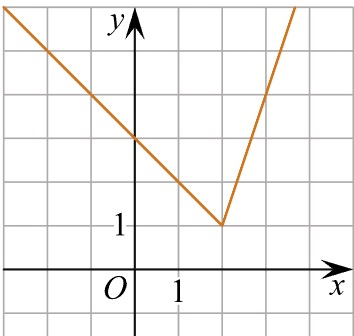
\includegraphics[align=t, width=\linewidth]{\picpath/K-L1}
		\end{minipage}
		%5
		\item
		\begin{minipage}[t]{\bodywidth}
			На рисунке изображён график функции вида \[ f(x)=ax-|bx+c|+d, \] где числа \(a, b, c, d\) --- целые.\\ Найдите корень уравнения \(ax+d=10\).
		\end{minipage}
		\hspace{0.02\linewidth}
		\begin{minipage}[t]{\picwidth}
			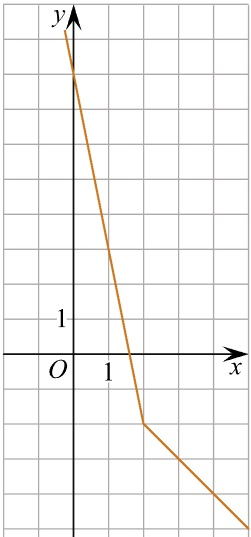
\includegraphics[align=t, width=\linewidth]{\picpath/K-L6}
		\end{minipage}
		%6
		\item
		\begin{minipage}[t]{\bodywidth}
			На рисунке изображён график функции вида \[ f(x)=ax+|bx+c|+d, \] где числа \(a, b, c, d\) --- целые.\\ Найдите корень уравнения \(ax+d=5\).
		\end{minipage}
		\hspace{0.02\linewidth}
		\begin{minipage}[t]{\picwidth}
			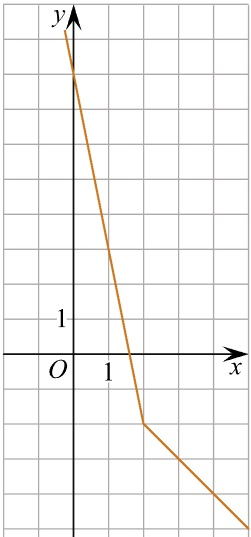
\includegraphics[align=t, width=\linewidth]{\picpath/K-L6}
		\end{minipage}
	\end{listofex}
\end{homework}
%END_FOLD

%BEGIN_FOLD % ====>>_ Домашняя работа 2 _<<====
\begin{homework}[number=2]
	\begin{listofex}
		\item ДЗ 2
	\end{listofex}
\end{homework}
%END_FOLD

%BEGIN_FOLD % ====>>_ Домашняя работа 3 _<<====
\begin{homework}[number=3]
	\begin{listofex}
		\item ДЗ 3
	\end{listofex}
\end{homework}
%END_FOLD

%BEGIN_FOLD % ====>>_ Проверочная работа _<<====
\begin{exam}
	\begin{listofex}
		\item Проверочная работа
	\end{listofex}
\end{exam}
%END_FOLD
